\begin{abstract}
Relative to zero cell, native target-cell conditioning in arbitrary-scale
super-resolution improves average quality but need not improve every image
or frequency band. We diagnose
this discrepancy through fixed-checkpoint corrections, separating amplitude
overshoot from wrong-direction changes using an exact squared-error identity.
A prospective replication on 32 natural images, LTE and an LTE-derived experimental variant under two
training seeds finds harmful corrections against both zero and nonzero cell
references. Relative to zero cell, native conditioning improves mean PSNR
in all four model--scale groups, yet uniform half-correction increases mean
RGB MSE by 0.26--7.55\%. A complete retrospective attenuation analysis
finds that even the HR-informed best uniform weight reduces this error
by at most .0011\% against zero and .086\% against the nonzero reference.
Nonzero references reveal additional failures and
change which images are labelled harmful: failure is a property of a specified
correction, not an intrinsic image label. Controlled high-frequency input
paths and equal-power phase changes further produce opposite gains at fixed
scale. The results quantify the limited repair capacity of uniform attenuation
and distinguish band damage from image-level and aggregate costs.
\end{abstract}
\begin{keywords}
Arbitrary-scale super-resolution, cell conditioning, frequency recovery,
readout failure analysis
\end{keywords}

\section{Introduction and Related Work}
\label{sec:intro}
Arbitrary-scale super-resolution (ASISR) predicts image values at continuous
coordinates. LIIF supplies target cell size to a local decoder
\cite{chen2021liif}; LTE introduces cell-dependent phase estimation
\cite{lee2022lte}. This information specifies the requested scale but does
not guarantee that the resulting output change reduces reconstruction
error. Our question is: \emph{what forms do harmful cell corrections take at a
fixed scale and band, and how much can reducing their amplitude repair?}
We measure failure types, damage magnitude and the cost of attenuation,
then test input changes that reverse benefit in controlled examples.

Harmful cell effects are not new. LIIF already varies cell size at fixed
queries; IPE-LIIF integrates positional features and reports cases where
an additional cell input hurts \cite{liu2021ipe}. Thera supplies analytic
Gaussian filtering and discusses its mismatch with bicubic training
\cite{becker2025thera}. Our fixed-checkpoint interventions are not a
performance comparison against these methods. Integrating intermediate
features also need not equal integrating a nonlinear decoder's RGB output.

Frequency-resolved analysis has precedents in HyRA's linear/nonlinear
responses \cite{fsds2024}, texture-based error analysis
\cite{magid2022texture}, sinusoidal degradation probes
\cite{kawai2026frequency}, and Nyquist-normalised forecasting
\cite{wang2026scaleanchoring}. The importance of phase beyond spectral
magnitude is classical \cite{oppenheim1981phase}. We do not claim these
principles, or the quadratic identity below, as new. Unlike architecture/retraining benchmarks \cite{nasir2026empirical},
we isolate inherited-checkpoint interventions.

Our empirical contributions are: (1) paired natural-image
measurements that separate image-level from band-level harm; (2) an
overshoot/direction diagnosis, using a classical error decomposition, with
a complete uniform-attenuation curve and its exact empirical optimum; and (3) controlled
input-path and fixed-power phase experiments that expose conditions hidden
by coarse frequency summaries. 

\section{Models and Evaluation Objects}
\label{sec:recovery}
\subsection{Keep the comparison fixed}
Natural-image tests use discrete HR targets and bicubic antialiased
LR observations. Changing supplied cell at fixed observation, query and
target measures a conditioning intervention, not a physical change of
pixel footprint. Native cell does not certify an exact pixel integral.

LTE and SC-INR inherit an EDSR-baseline encoder, DIV2K training
\cite{agustsson2017div2k}, a 256-dimensional representation, an MLP with three
256-unit hidden layers, 1000 epochs and scales $\times1$--$\times4$.
SC-INR is our earlier LTE-derived experimental variant, not an independent
model family or a new performance method proposed here. LTE conditions
Fourier phase on cell. SC instead predicts frequency $\omega_k(z)$ and
phase from image features $z$, and multiplies its sine/cosine features by
\begin{equation}
 w_k(c_{\rm rel})=\operatorname{sinc}(\omega_{kx}c_{{\rm rel},x}/2)
        \operatorname{sinc}(\omega_{ky}c_{{\rm rel},y}/2),
 \label{eq:sc}
\end{equation}
where $\operatorname{sinc}(v)=\sin(\pi v)/(\pi v)$ and
$c_{\rm rel}=c\,n_{\rm LR}$ is cell in LR-feature units. Its 128 frequencies use a signed $2.1\tanh$ parameterisation;
cell enters only through $w_k$ before the nonlinear MLP. This does not
make the final RGB output an exact pixel integral. The variants differ
in phase and frequency parameterisation as well as cell response, so
between-model differences cannot isolate the causal effect of sinc.

A retrained no-readout ablation changes weights; our cell interventions
preserve weights, observations and queries. Earlier probes use seed1;
the new natural-image replication uses inherited seeds 1 and 2. The LTE
snapshots omit the original extrapolation cell clamp. Zero cell lies
outside training support. We compare failure behaviour rather than claim
an architecture advantage.

\section{Failure Types and Attenuation Limits}
\label{sec:failure}
\subsection{Overshoot and wrong direction}
For fixed-weight outputs, let $F_c$ be native-cell prediction, $F_r$
a declared reference-cell prediction, $t$ the HR target, and $d=F_c-F_r$. Inner products
are pixel/channel means, optionally after band projection. Set
$a=\langle t-F_r,d\rangle$, $b=\|d\|^2$ and
\begin{equation}
 G(\lambda)=\operatorname{MSE}(F_r,t)-\operatorname{MSE}(F_r+\lambda d,t)
             =2\lambda a-\lambda^2b.
 \label{eq:gain}
\end{equation}
For a harmful native correction $G(1)<0$ and $b>0$, $0<a<b/2$ is
\emph{overshoot}: a smaller positive correction can help. When $a<0$,
the \emph{direction is wrong}: every positive multiple hurts. The unconstrained oracle
optimum is $\lambda^*=a/b$. This classical identity diagnoses saved
outputs using HR truth; output interpolation is not a cell intervention
or an observation-only method. We define harm by $G(1)<-10^{-8}$. For the saved natural outputs,
$b$, $|a|$ and $|a-b/2|$ within
$64\epsilon_{64}\max(\operatorname{MSE}(F_r,t),b,10^{-8})$
are retained as numerical boundaries; $\epsilon_{64}$ is machine precision.

\subsection{Prospective natural-image replication}
We freeze a new cohort, DIV2K valid0837--0868, before inference: 32 images,
LTE/SC seeds 1 and 2, and $\times2/4$. This excludes previous development, forecast and checkpoint-validation
images. The centre HR128 target and bicubic-AA
LR observation are held fixed. Each checkpoint predicts four supplied
relative cells $c_{\rm rel}=c\,n_{\rm LR}\in\{0,1/2,2/3,1\}$; native
is 1 at $\times2$ and $1/2$ at $\times4$. Training uses LR48 and integer
HR48--192, so all three nonzero values occur in the training cell's
numeric support. Changing cell at a fixed target remains mismatched
conditioning, not a joint in-distribution sample or physical target change.

All 1024 RGB predictions are hash-frozen before target scoring. Unless
stated otherwise, metrics use raw RGB in units of the unit-range target,
after removing a four-pixel border (shave4); outputs are not clipped. The primary
contrasts are native versus zero and native versus $c_{\rm rel}=2/3$
(denoted $h3$); the other nonnative contrasts are retained. Three non-DC
Chebyshev bands use cutoffs $1/8,1/4,1/2$ on the shaved RGB channels,
with pixel-domain normalisation. Image-cluster bootstrap resamples all
32 images jointly across seeds, 10,000 times, with pointwise intervals;
repeated seeds and scales are not additional independent images.

\begin{table}[t]\centering
\caption{Prospective natural-image replication. Each row has 64 RGB and
192 band records (32 images, two seeds). RGB: all negative records
followed by those losing $>.01$ dB in parentheses. Band O/D: overshoot/
wrong-direction counts. $\Delta E_{1/2}$: half-correction mean RGB MSE
change relative to native, over all cases.}
\label{tab:failures}
\small
\begin{tabular}{lccrrr}\toprule
Model & $s$ & Ref. & RGB & Band O/D & $\Delta E_{1/2}$\\\midrule
LTE & 2 & zero & 1 (1) & 5/1 & +7.55\%\\
 & 2 & $h3$ & 13 (6) & 13/11 & +2.29\%\\
 & 4 & zero & 2 (1) & 18/2 & +2.77\%\\
 & 4 & $h3$ & 35 (10) & 21/84 & $-.058$\%\\\midrule
SC & 2 & zero & 10 (5) & 10/12 & +5.46\%\\
 & 2 & $h3$ & 17 (9) & 13/16 & +1.84\%\\
 & 4 & zero & 11 (5) & 17/30 & +.264\%\\
 & 4 & $h3$ & 25 (7) & 11/83 & +.087\%\\\bottomrule
\end{tabular}
\end{table}

\textbf{Average benefit coexists with individual harm.}
Against zero, mean native-minus-reference PSNR is $.912/.444$ dB for
LTE at $\times2/4$ and $.687/.028$ dB for SC; all four 95\% image-bootstrap
intervals are above zero. Yet Table~\ref{tab:failures} contains negative
cases in every group. The nonzero $h3$ contrast also has harmful images
in both seeds of each model and scale, so harm is not confined to zero-cell
probes. At $\times4$, 35/64 LTE and 25/64 SC RGB records are negative,
but only 10 and 7 lose more than $.01$ dB; worst losses are $.202$ and
$.136$ dB. Counts and effect sizes answer different questions.

\textbf{Failure identity depends on the correction.}
SC at $\times2$ retains all ten zero-reference negative RGB records
against $h3$. At $\times4$, its eleven zero-reference failures and
25 $h3$ failures are disjoint. Here the references lie on opposite sides
of native cell.  Across the two training seeds, zero-reference SC RGB harm
repeats in 10/11 image--scale cases harmed by either seed; LTE repeats in
1/2. Against $h3$, the corresponding overlaps are 17/25 and 19/29.
Failure types occur repeatedly, but exact labels and their prevalence
cannot be assigned permanently to a model or image.

\textbf{How much can uniform attenuation repair?}
After the original replication, we reanalyse all saved outputs over
$\lambda=0,.01,\ldots,1$ (Fig.~\ref{fig:attenuation}). This is retrospective,
not another prospective test. With $A=\operatorname{mean}(a)$ and
$B=\operatorname{mean}(b)$, the exact empirical best uniform weight is
$\hat\lambda=\operatorname{clip}(A/B,0,1)$. Against zero, it is 1 for
LTE at both scales and SC at $\times4$, and .9931 for SC at $\times2$:
the largest mean-MSE reduction from native is only .0011\%.
Against $h3$, the respective LTE/SC $\times2/4$ optima are
$.9878/.6809$ and $.9602/.8908$, with improvements
$.0014/.0853\%$ and $.0138/.0074\%$. Even separate HR-informed per-record
weights reduce mean RGB MSE by at most .072\% (zero) and .298\% ($h3$).
These are empirical ceilings for the declared output-interpolation family,
not deployable policies or bounds on other corrections. They show that
uniform attenuation has little repair capacity in this cohort; a few
rescued cases alone overstate its practical value.

\begin{figure}[t]\centering
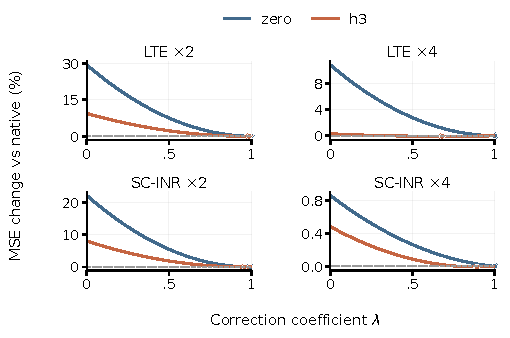
\includegraphics[width=\columnwidth]{figures/attenuation.pdf}
\caption{Complete uniform output-attenuation curves, all 32 images and
both seeds. Zero is native mean MSE; lower is better. Dots mark the
exact HR-informed group optima, not a deployable selected method.
Panels use different vertical ranges.}
\label{fig:attenuation}
\end{figure}

\textbf{Metric sensitivity and visible magnitude.}
Six fixed retrospective conventions cross raw or $[0,1]$-clipped endpoints
with 0/4/8-pixel borders. Clipping is applied before interpolation, not
after. Every convention retains mean benefit over zero and overall harm
from half-correction: MSE increases span 7.55--7.67\% (LTE$\times2$),
2.66--2.94\% (LTE$\times4$), 5.17--5.49\% (SC$\times2$) and
.226--.264\% (SC$\times4$). Negative counts vary (SC$\times2$: 5--10/64;
LTE$\times4$: 1--3/64), so stable aggregate conclusions do not imply
stable labels. The largest best-uniform improvement across all six
conventions remains .0016\% against zero and .086\% against $h3$.
Fig.~\ref{fig:examples} shows prespecified median-loss examples with a
common error-change scale, rather than visually selected worst cases.

\begin{figure*}[t]\centering
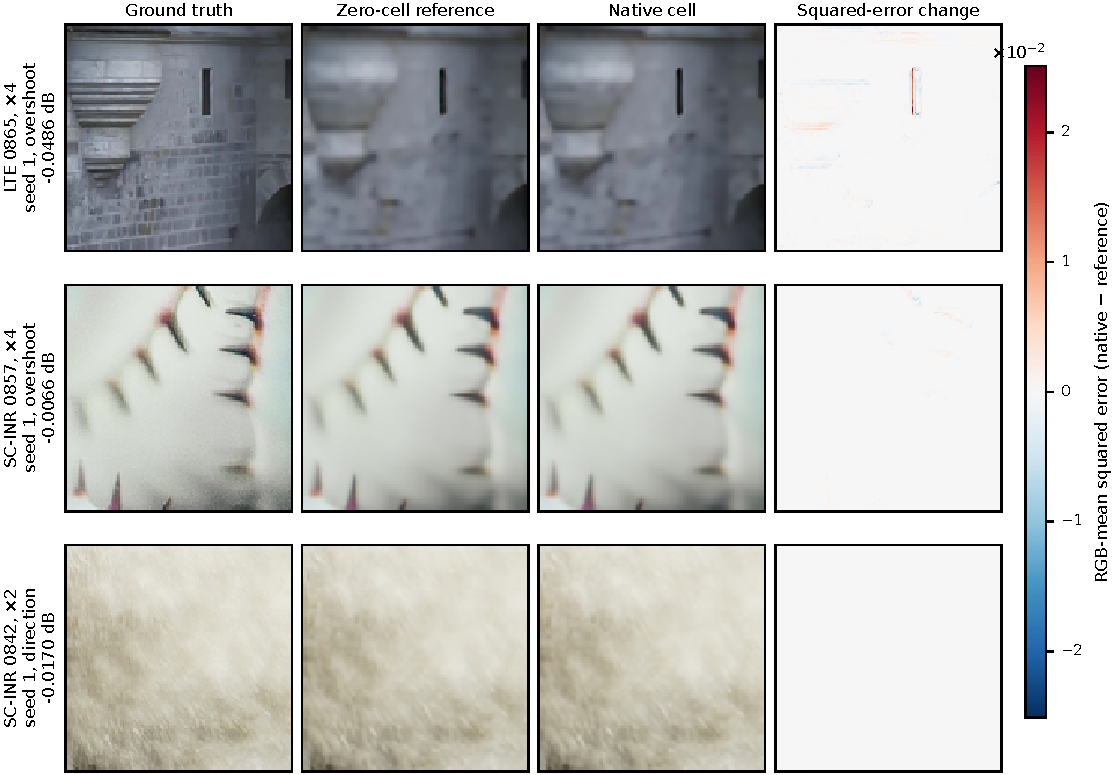
\includegraphics[width=.80\textwidth]{figures/natural-median.pdf}
\caption{Natural-image harm against zero cell. For each available
model/failure class, the record nearest its median RGB PSNR loss is
selected (ties: image, seed, scale); LTE has no wrong-direction RGB
failure in this cohort. All images show the same shave4 region. The
squared-error-change maps use a common scale; positive means native
worsens error. Small PSNR losses need not be visibly obvious.}
\label{fig:examples}
\end{figure*}

\textbf{Cell gain is not absolute model quality.}
On the same 32 images, native RGB PSNR averaged over both seeds is
34.080/34.054 dB (LTE/SC, $\times2$) and 29.033/29.045 dB ($\times4$).
Paired SC-minus-LTE differences are $-.0253$ dB (95\% image-bootstrap
interval $[-.0576,-.0002]$) and $+.0119$ dB ($[-.0156,.0437]$).
SC wins on 13/32 and 20/32 seed-averaged images. These small mixed
checkpoint differences support neither uniform LTE dominance nor a new
SC performance claim. SC supplies a contrasting feature-level cell design
within the LTE lineage.

\section{Controlled Input-Path and Phase Experiments}
\label{sec:controlled}
\subsection{Design: separate two interventions}
We fix seed1 checkpoints and $\times4$. A monochrome HR64 target,
replicated across RGB, is $t=.5+L+H$. The low modes are
$L=\{(2,0),(0,2),(2,2)\}$; the four high templates are
\begin{align*}
 M_a&=\{(10,0),(12,0),(14,0)\},\\
 M_c&=\{(10,0),(0,12),(10,10)\},\\
 H_a&=\{(18,0),(22,0),(26,0)\},\\
 H_c&=\{(18,0),(0,22),(18,18)\}.
\end{align*}
All cosine amplitudes are $.04$; frequencies are cycles per 64 pixels,
above LR Nyquist (8). A low-frequency sham uses
$\{(4,0),(0,4),(4,4)\}$. Four high-branch phase vectors (zero plus three
uniform vectors, seed 20261012) cross four translations
$\{0,.5\}^2$ in LR-pixel units. Low initial phases are zero; translations
move both branches. A periodic separable bicubic-AA operator $A$ produces
LR16 observations
\begin{equation}
 y_\eta=A(.5+L)+\eta A(H),\quad\eta\in\{0,.5,1\}.
 \label{eq:path}
\end{equation}
The sham always uses $At$. Changing $\eta$ holds the target fixed but also
changes LR energy and gradients; it is not a pure aliasing intervention.
Changing high-branch phase instead holds each target Fourier magnitude
fixed. Primary centre32 and sensitivity full64 both contain integer
periods. No clipping is used; the same three non-DC bands are scored.
Gain ties use $10^{-8}$, alignment boundaries $10^{-10}$ and tiny-change
energy $10^{-12}$. The 240 conditions contain 148 unique inputs and
296 native/zero pairs; outputs were frozen before scoring. These are
controlled examples, not independent natural images.

\subsection{Alignment reversals and fixed-power counterexamples}
For the two middle-frequency templates (32 phase--position conditions),
increasing $\eta$ from 0 to 1 lowers middle-band gain in 29/32 LTE and
32/32 SC conditions. Harmful outcomes increase from 18 to 32 and 15 to
31, respectively; 14/32 and 16/32 change from positive to negative
alignment $a$. Full64 evaluation retains gain decreases in 31/32 for
both models, although exact negative counts change. The high-frequency
templates instead contain both signs of path effect
across the fixed grid; the path is not uniformly harmful.

At $\eta=1$, changing phase at fixed template and position produces both
positive and negative high-band gains in all eight template--position
groups per model, in both evaluation regions. Thus \emph{target power
alone does not determine readout benefit in these fixed models}.
This does not hold LR power/gradients fixed. At $\eta=0$, high-phase
variants share identical inputs and outputs: score differences then
reflect different unobserved targets, not a neural response to hidden
phase. These distinctions prevent phase sensitivity from being mistaken
for a general adaptive mechanism.

Effects are small: at $\eta=1$ in the high templates, centre-region
full-RGB native-minus-zero PSNR spans $[-.00730,.01236]$ dB for LTE and
$[-.00164,.000891]$ dB for SC. Sign reversals provide diagnostic
counterexamples, not a practical performance advance or an estimate
of natural-image causal prevalence.

\section{Guidance, Scope and Conclusion}
\label{sec:limits}
\textbf{Operational boundary.}
The diagnosis uses HR truth. Replacing it by bicubic interpolation leaves
the unknown term $2\langle t-B(y),d\rangle$; this is not an unbiased
risk estimator like generalized SURE under its stated assumptions
\cite{eldar2008gsure}. In a preceding held-out forecast, adding this proxy
to a magnitude/spectrum baseline detects the same 6/14 harmful SC bands
but increases false positives from 15 to 17. A useful observation-only
rule remains unestablished.

\textbf{Scope and cost.}
Evidence covers LTE and its SC derivative, not independent families.
The finite periodic probes do not identify natural-image causal prevalence;
nonzero controls establish numeric cell support only. No matching training
was performed. The replication, independent scoring audit and retrospective
closure took 637.27, 6.88 and 11.08 seconds on one CPU thread, with no GPU.

\textbf{Conclusion.}
Native cell conditioning improves average reconstruction against zero,
while individual corrections can overshoot or move away from the target.
Nonzero references and training seeds reproduce failures but change their
identities. Complete attenuation curves reveal little empirical repair
capacity within the output line segment; fixed-power phase examples show
why band energy alone cannot determine benefit. Readout assessment should
report the specified contrast, failure type, actual image-level damage and
aggregate cost of repair.

\section{Acknowledgments}
Claude and OpenAI Codex assisted with text, analysis code, figures and
record checks. Numerical records were audited; human author review and
responsibility are required before submission.
